\documentclass{beamer}
\usepackage{hyperref}
\usepackage[CJKmath=true, AutoFakeBold = true]{xeCJK}
% \usepackage[T1]{fontenc}
\setCJKmainfont{AR PL KaitiM GB}
\usepackage{latexsym,xcolor,multicol,booktabs,calligra}
\usepackage{amssymb,amsfonts,amsmath,amsthm,mathrsfs,mathptmx}
\usepackage{graphicx,pstricks,listings,stackengine}
\usepackage[most]{tcolorbox}
\usefonttheme[onlymath]{serif}
\usepackage[brazil]{babel}

\renewcommand{\today}{29 de Junho de 2023}
\renewcommand{\alert}[1]{\textbf{\color{swufe}#1}}

\author[Rodrigues, J.]{Julio Cesar da Silva Rodrigues\inst{1}}
\title[Modelagem Computacional - TP]{Análise de Abordagens Distintas na Modelagem de Crescimento de Tumores com EDOs}
\institute[UFSJ]
{
    \inst{1} 
    Universidade Federal de São João del-Rei \\
    Curso de Ciência da Computação \\
    \textit{julio.csr.271@aluno.ufsj.edu.br}\\
    \vspace{0.35cm}
}

\date{29 de Junho de 2023}
\usepackage{SWUFE}

\def\cmd#1{\texttt{\color[RGB]{0, 0, 139}\footnotesize $\backslash$#1}}
\def\env#1{\texttt{\color[RGB]{0, 0, 139}\footnotesize #1}}

\lstset{
    language=[LaTeX]TeX,
    basicstyle=\ttfamily\footnotesize,
    keywordstyle=\bfseries\color[RGB]{0, 0, 139},
    stringstyle=\color[RGB]{50, 50, 50},
    numbers=left,
    numberstyle=\small\color{gray},
    rulesepcolor=\color{red!20!green!20!blue!20},
    frame=shadowbox,
}

\begin{document}

\begin{frame}
    \titlepage
    \vspace*{-1.5cm}
    \begin{figure}[htpb]
        \begin{center}
            
\includegraphics[width=0.4\linewidth]{pic/LogoUFSJ.PNG}
        \end{center}
    \end{figure}
\end{frame}

\begin{frame}
    \tableofcontents[sectionstyle=show,subsectionstyle=show/shaded/hide,subsubsectionstyle=show/shaded/hide]
\end{frame}

\section{Introdução}

\begin{frame}{Recapitulando}

    \begin{itemize}
        \setlength{\itemsep}{10pt}
        \item Estudo baseado no modelo de Simeoni et al. \cite{tu};
        \item Bem-sucedido na modelagem de crescimento de tumores;
        \item Considera que a ação de medicamentos não é instantânea;
        \item Proposta de uma alternativa com EDOs de atraso;
        \item Testes com crescimento de tumor mamário em ratos.
    \end{itemize}
    
\end{frame}

\section{Sistemas de EDOs}

\begin{frame}{Modelo de Simeoni}
    
    \begin{block}{Função de Crescimento de Tumor (\(TGF\))}
        \begin{equation*}
            TGF(t) = \frac{\lambda_0 \cdot Z_1(t)}{\left[1 + \left(\frac{\lambda_0}{\lambda_1} \cdot V(t)\right)^\psi\right]^{\frac{1}{\psi}}}
        \end{equation*}
    \end{block}
    
    \begin{block}{Compartimento \(Z_1\)}
        \begin{equation*}
            \frac{dZ_1(t)}{dt} = TGF(t) - k_1 \cdot c(t) \cdot Z_1(t)
        \end{equation*}
    \end{block}
    
\end{frame}

\begin{frame}{Modelo de Simeoni}

    \begin{block}{Compartimento \(Z_2\)}
        \begin{equation*}
            \frac{dZ_2(t)}{dt} = k_1 \cdot c(t) \cdot Z_1(t) - k_2 \cdot Z_2(t)
        \end{equation*}
    \end{block}

    \begin{block}{Compartimento \(Z_3\)}
        \begin{equation*}
            \frac{dZ_3(t)}{dt} = k_2 \cdot Z_2(t) - k_2 \cdot Z_3(t)
        \end{equation*}
    \end{block}

    \begin{block}{Compartimento \(Z_4\)}
        \begin{equation*}
            \frac{dZ_4(t)}{dt} = k_2 \cdot Z_3(t) - k_2 \cdot Z_4(t)
        \end{equation*}
    \end{block}
    
\end{frame}

\begin{frame}{Modelo de Simeoni}

    \begin{figure}
        \centering
        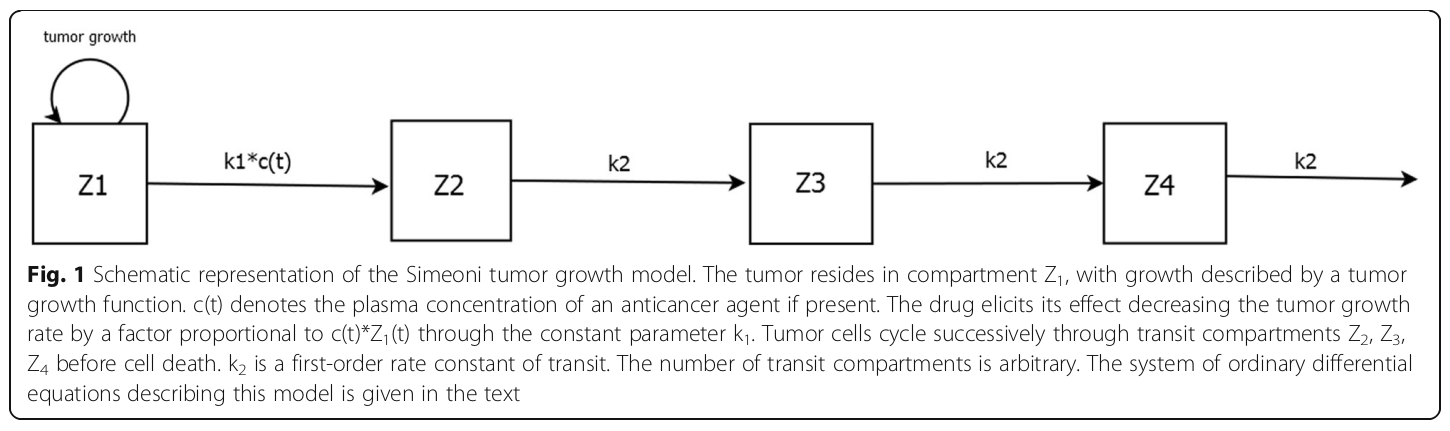
\includegraphics[width=0.9\textwidth]{pic/simeoni.png}
        \hspace*{15pt}\hbox{\scriptsize Fonte:\thinspace{\small \scriptsize{(Koziol et al., 2020, Pág. 2)}\footnotemark}}\\
        \label{fig:map1}
    \end{figure}

    \begin{itemize}
        \setlength{\itemsep}{10pt}
        \item Geralmente, o número de compartimentos é arbitrário.
    \end{itemize}
    
    \footnotetext[1]{\tiny{Disponível em: \url{https://bmccancer.biomedcentral.com/articles/10.1186/s12885-020-6703-0}}}
\end{frame}

\begin{frame}{Modelo Alternativo}
    
    \begin{block}{Compartimento \(Z_1\)}
        \begin{equation*}
            \frac{dZ_1(t)}{dt} = TGF(t) - k_1 \cdot c(t) \cdot Z_1(t)
        \end{equation*}
    \end{block}

    \begin{block}{Compartimento \(Z_2\)}
        \begin{equation*}
            \frac{dZ_2(t)}{dt} = k_1 \cdot c(t) \cdot Z_1(t) - k_2 \cdot delay(Z_2, t_2)
        \end{equation*}
    \end{block}

    \begin{itemize}
        \setlength{\itemsep}{10pt}
        \item \(t_2\) representa o atraso de tempo antes da eliminação.
    \end{itemize}
    
\end{frame}

\begin{frame}{Modelo Alternativo}

    \begin{figure}
        \centering
        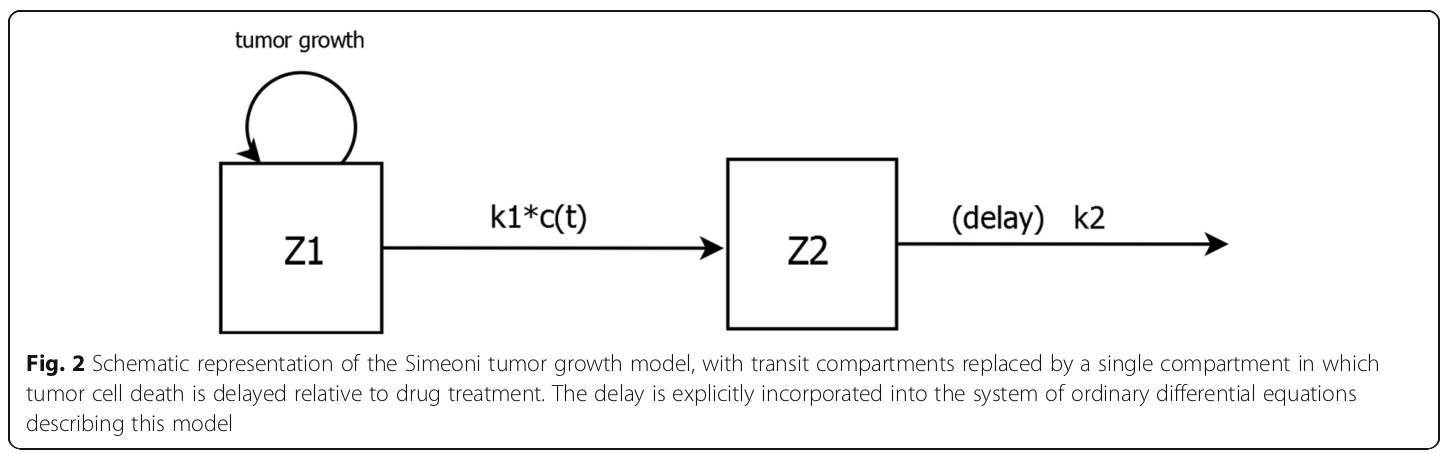
\includegraphics[width=0.9\textwidth]{pic/proposal.png}
        \hspace*{15pt}\hbox{\scriptsize Fonte:\thinspace{\small \scriptsize{(Koziol et al., 2020, Pág. 2)}\footnotemark}}\\
        \label{fig:map2}
    \end{figure}
    
    \footnotetext[2]{\tiny{Disponível em: \url{https://bmccancer.biomedcentral.com/articles/10.1186/s12885-020-6703-0}}}
\end{frame}

\section{Metodologia}

\begin{frame}{Base de Dados}
    
    \begin{itemize}
        \setlength{\itemsep}{10pt}
        \item Observações no crescimento de tumor em 40 ratos:
        \begin{enumerate}
            \vspace{0.2cm}
            \setlength{\itemsep}{10pt}
            \item 21 sem tratamento;
            \item 19 com tratamento.
        \end{enumerate}
        \item Todos os animais saudáveis no primeiro dia;
        \item Dose única de \emph{cisplatin} no início da experimentação.
    \end{itemize}
    
\end{frame}

\begin{frame}{Implementações}
    
    \begin{itemize}
        \setlength{\itemsep}{10pt}
        \item Artigo:
        \begin{enumerate}
            \vspace{0.2cm}
            \setlength{\itemsep}{10pt}
            \item NLME\footnotemark \hspace{0.1cm}para ajustar as curvas de crescimento;
            \item Monolix 2019R1 com SAEM\footnotemark \hspace{0.1cm}para estimar parâmetros.
        \end{enumerate}
        \item Presente trabalho:
        \begin{enumerate}
            \vspace{0.2cm}
            \setlength{\itemsep}{10pt}
            \item Evolução diferencial;
            \item Comparação de simulações com ambos sistemas de EDOs.
        \end{enumerate}
    \end{itemize}

    \footnotetext[3]{\tiny{Nonlinear Mixed Effects}}
    \footnotetext[4]{\tiny{Stochastic Approximation Expectation Maximization}}
    
\end{frame}

\begin{frame}{Exemplo\nocite{my}}

    \begin{figure}
        \centering
        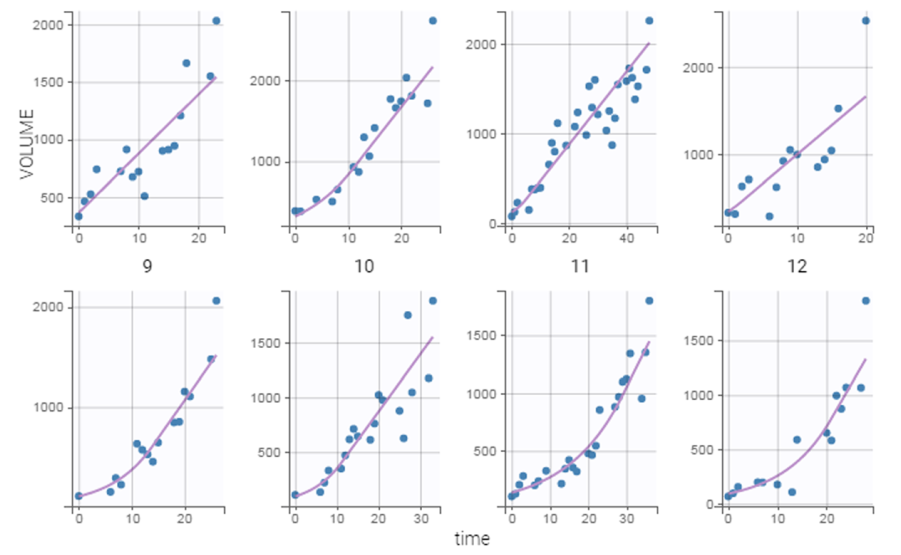
\includegraphics[width=0.85\textwidth]{pic/s_fit.png}
        \hspace*{15pt}\hbox{\scriptsize Fonte:\thinspace{\small \scriptsize{(Koziol et al., 2020, Pág. 5)}\footnotemark}}\\
        \label{fig:map3}
    \end{figure}
    
    \footnotetext[5]{\tiny{Disponível em: \url{https://bmccancer.biomedcentral.com/articles/10.1186/s12885-020-6703-0}}}
    
\end{frame}

\section{Limitações}

\begin{frame}{Dificuldades Encontradas}
    
    \begin{itemize}
        \setlength{\itemsep}{10pt}
        \item Escolha de valores da \emph{TGF};
        \item Interpretação da base de dados;
        \item Calibragem do algoritmo.
    \end{itemize}
    
\end{frame}

\section*{Final}

\begin{frame}{Referências}
    \scriptsize\bibliographystyle{apalike}
    \bibliography{ref}
\end{frame}

\end{document}